\begin{table*}[]
\centering
\caption{Summary of results for \textit{bmi\_refresh}, \textit{static\_batch},
\textit{partial\_refresh} and \textit{precision\_strategy}}
\label{table.summary}
\begin{tabular}{|c|c|c|c|c|c|}
\hline
\textbf{Strategy} & \begin{tabular}[x]{@{}c@{}}
    \textbf{Avg. Recall}\\ \textbf{@($E_{norm}$=1)}
\end{tabular} & \begin{tabular}[x]{@{}c@{}}
\textbf{Avg. Recall}\\ \textbf{@($E_{norm}$=1.5)}
\end{tabular} & \begin{tabular}[x]{@{}c@{}}
\textbf{Avg. Recall}\\ \textbf{@($E_{norm}$=2)}
\end{tabular} & \textbf{$E_{norm}$ for 75\% recall} &
\begin{tabular}[x]{@{}c@{}}
    \textbf{Running Time}\\ \textbf{(in min)}
\end{tabular} \\ \hline \hline
bmi\_refresh & 0.715 & 0.827 & 0.905 & 1.128 & 0.22 \\ \hline \hline
static\_batch($k=1$) & 0.750 & 0.865 & 0.926 & 1.021 & 49.29 \\ \hline
static\_batch($k=100$) &  0.704 & 0.807 & 0.887 & 1.167 & 0.47 \\ \hline \hline
partial\_refresh($k=10$,$s=1000$) &  0.753 & 0.862 & 0.926 & 1.008 & 40.92 \\ \hline
partial\_refresh($k=100$,$s=500$) &  0.753 & 0.855 & 0.923 & 1.022 & 38.28 \\ \hline
partial\_refresh($k=100$,$s=1000$) &  0.754 & 0.856 & 0.922 & 1.013 & 39.57 \\ \hline
partial\_refresh($k=100$,$s=5000$) &  0.756 & 0.855 & 0.921 & 1.016 & 40.70 \\ \hline
partial\_refresh($k=500$,$s=1000$) &  0.700 & 0.785 & 0.815 & 1.324 & 38.63\\
\hline \hline
precision\_strategy($m=25$,$p=0.4$) &  0.698 & 0.849 & 0.915 & 1.129 & 35.68 \\ \hline
precision\_strategy($m=25$,$p=0.6$) &  0.735 & 0.859 & 0.923 & 1.059 & 40.20 \\ \hline
precision\_strategy($m=25$,$p=0.8$) &  0.750 & 0.862 & 0.926 & 1.024 & 44.64 \\ \hline
precision\_strategy($m=25$,$p=1.0$) &  0.752 & 0.865 & 0.926 & 1.014 & 47.41 \\
\hline
% recency\_weighting($w=1$,$it=1000$) &  0.704 & 0.798 & 0.875 & 1.243 & 11.75 \\ \hline
% recency\_weighting($w=2$,$it=1000$) &  0.705 & 0.806 & 0.884 & 1.219 & 11.66 \\ \hline
% recency\_weighting($w=5$,$it=1000$) &  0.704 & 0.814 & 0.887 & 1.191 & 11.63\\ \hline
% recency\_weighting($w=10$,$it=1000$) &  0.707 & 0.824 & 0.891 & 1.206 & 11.54\\ \hline
\end{tabular}
\end{table*}

For sake of space and readability, we encode each strategy with their parameter
settings as \textit{strategy\_name($param1=x,\ldots$)}. Table~\ref{table.strategies}
lists all the strategies and their parameters. Table~\ref{table.summary} lists
the results for different parameter settings of \textit{bmi\_refresh}, \textit{static\_batch},
\textit{partial\_refresh} and \textit{precision\_strategy}.
We report the recall achieved at different values of effort, effort required to
achieve $75\%$ recall, and the average running time. Instead of absolute effort,
we use normalized effort $E_{norm}$ as defined in Section~\ref{sec.dataeval}. For
example, ``Avg. recall@($E_{norm}=1.5$)'' denotes the average recall achieved
across all the topics when $1.5 \times R$ documents haven been judged, where $R$
is the total number of relevant documents for a topic.

With \textit{static\_batch}($k = 1$), CAL achieves significantly higher recall of
$75\%$ at $E_{norm} = 1$ than \textit{bmi\_refresh} which achieves $71.5\%$
recall.  \textit{static\_batch}($k = 100$) performs worse than
\textit{bmi\_refresh}, managing to achieve $70.4\%$ recall at the same effort.
These results establish that frequent refreshing helps to achieve higher recall.
Although the batch sizes in BMI increases exponentially with time, it still does
frequent refreshes during the early stages of the CAL process, thus performing
better than \textit{static\_batch($k = 100$)}. \textit{bmi\_refresh} is also
extremely cheap in terms of computation cost since it only performs a
logarithmic number of refreshes relative to \textit{static\_batch} strategies.
\textit{bmi\_refresh} simulation finished in less than a minute while
\textit{static\_batch}($k=1$) took $49$ minutes.

We evaluate rest of the refresh
strategies by comparing them to \textit{static\_batch}($k = 1$).

By fixing $s=1000$ and varying $k$ in \textit{partial refresh strategy}, we observe
that for $k=10$ and $k=100$, the difference in recall remains insignificant throughout the
CAL process. Their recall scores are also very similar to
\textit{static\_batch}($k = 1$). They achieve $86.2\%$ and $85.5\%$ recall at
$E_{norm} = 1.5$, respectively. For $k=500$, we observe $78.6\%$ recall at the
same effort, which is worse than \textit{bmi\_refresh} ($82.6\%$). This is in
agreement with our previous observation that more frequent full refreshes
increases CAL's effectiveness. \textit{static\_batch}($k=100$) 
consistently achieved lower recall when compared to \textit{static\_batch}($k = 1$) while
\textit{partial\_refresh}($k=100,s=1000$) is as effective as the latter. Based
on this, it can be established that partial refreshing contributes significant
improvements to recall. On fixing $k = 100$ and varying $s$ we observe no changes to the
recall values. \textit{Partial refresh strategies} also improve the running time
of simulations by $20\%$ when compared to \textit{static\_batch}($k = 1$).

In \textit{precision based refresh strategy}, we fix $m = 25$ and vary $p$. For
$p=0.8$ and $p=1.0$, \textit{precision\_strategy} achieves $75\%$ recall at
$E_{norm} = 1$ which is similar to \textit{static\_batch($k = 1$)}. This
similarity of recall is also seen at $E_{norm} = 1.5$ and $E_{norm} = 2$. When
$p=1$, \textit{precision\_strategy} refreshes whenever a non-relevant judgment
is made, thus behaving very similar to \textit{static\_batch}($k = 1$). For
lower values of $p$, we observe lower recall values during the initial stages
($73.5\%$ recall when $E_{norm} = 1$ for $p=0.6$). However, they catch up to
\textit{static\_batch}($k = 1$) at higher $E_{norm}$, as relevant documents
become rarer ($85.9\%$ recall when $E_{norm} = 1.5$ for $p=0.6$).
\textit{precision\_strategy} improved the running time of simulations by $15\%$
on average when compared to \textit{static\_batch}($k = 1$).
\textit{precision\_strategy} triggers lower number of refreshes during the
beginning of the CAL process when relevant documents are easier to find. During
the later stages when the relevant documents are harder to find,
$precision\_strategy$ tends to keep refreshing after every judgment. 

During our initial experiments, \textit{recency\_weighting} seemed to have no
impact on the recall values. On further experiments, we found that the default
number of training iterations ($it=100000$) was very high for recency
weighting to cause any difference. By reducing the number of training iterations
to $1000$, we introduced significant degradation in the system's effectiveness.
Reducing the number of training iterations also
reduced the running time of simulation by $76\%$ when compared to
\textit{static\_batch}($k = 1$). We used \textit{recency\_weighting} to see
whether it could recover the lost effectiveness.
\textit{recency\_weighting}($w=1,it=1000$) is equivalent to
\textit{static\_batch}($k=1,it=1000$) and it achieves $70.4\%$ and $79.8\%$
recall when $E_{norm}$ is equal to $1$ and $1.5$ respectively. By increasing
$w$, we observe an increase in recall for $E_{norm} \in \{1.5, 2\}$. However,
the recall is consistently and significantly lower when compared to
\textit{static\_batch}($k=1$). For example,
\textit{recency\_weighting}($w=10,it=1000$) is only able to achieve $82.4\%$
recall at $E_{norm}=1.5$.

% \begin{figure}
%  \centering 
%  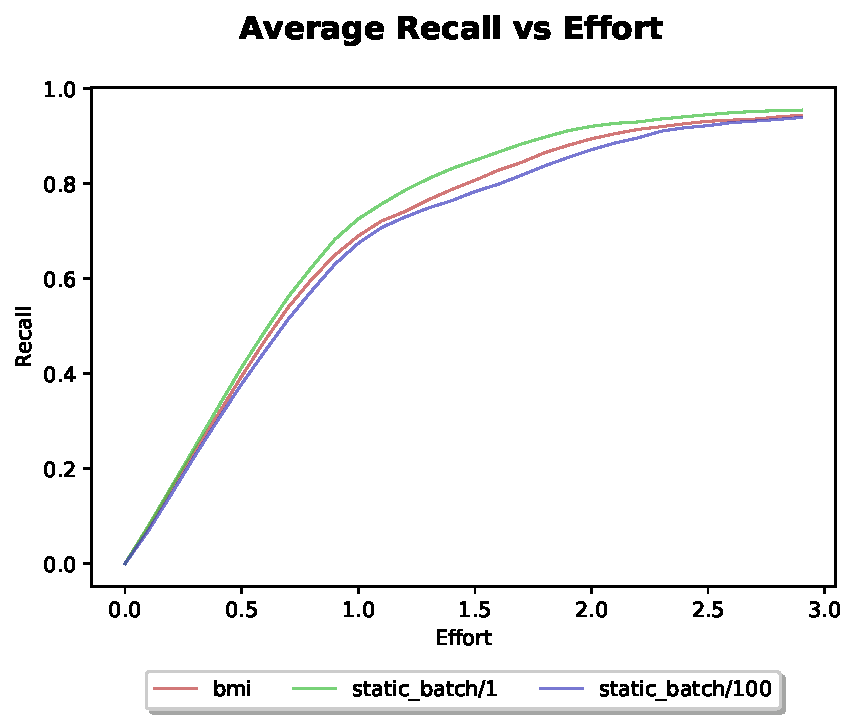
\includegraphics[width=1.0\linewidth]{static1.pdf}
%  \caption{Static Refresh}
%  \label{fig.static1}
% \end{figure}

% \begin{figure}
%  \centering 
%  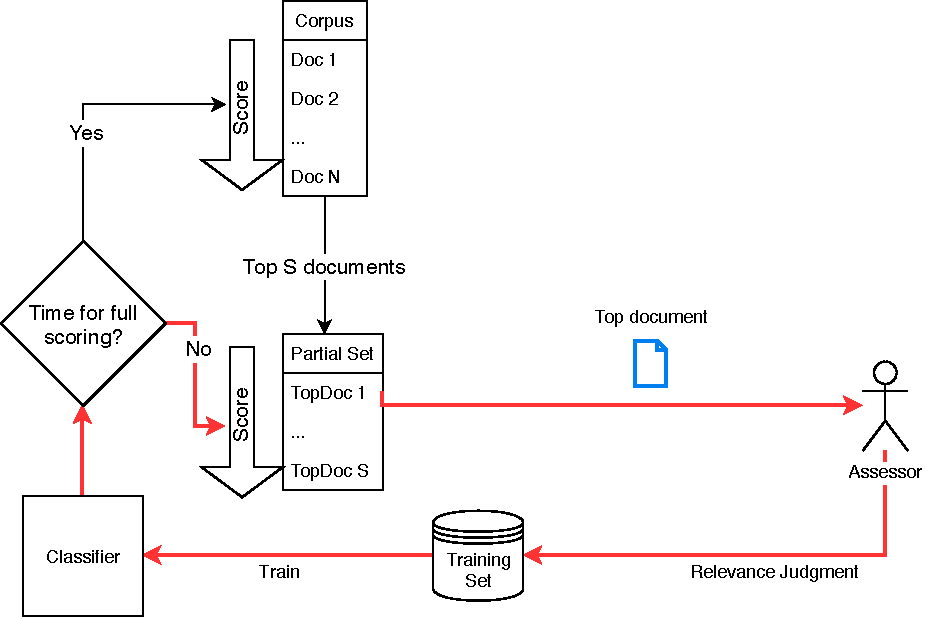
\includegraphics[width=1.0\linewidth]{partial1.pdf}
%  \caption{Partial Refresh}
%  \label{fig.partial1}
% \end{figure}

% \begin{figure}
%  \centering 
%  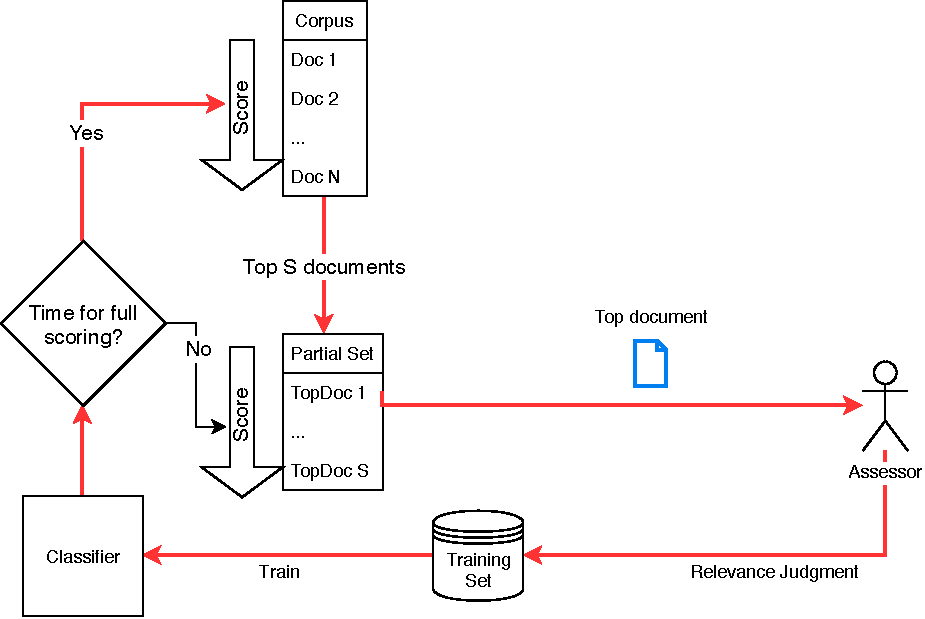
\includegraphics[width=1.0\linewidth]{partial2.pdf}
%  \caption{Partial Refresh}
%  \label{fig.partial2}
% \end{figure}

% \begin{figure}
%  \centering 
%  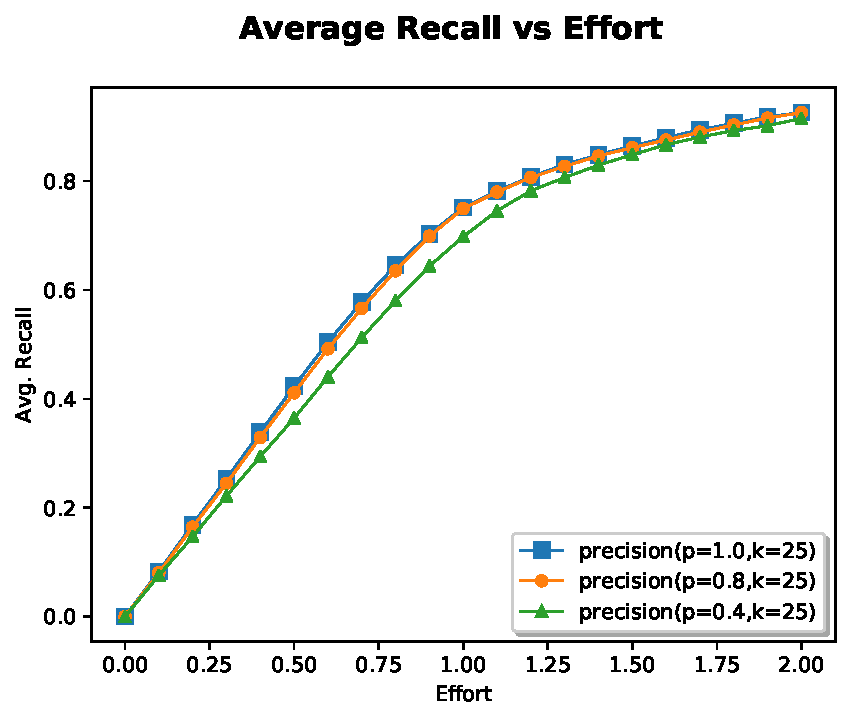
\includegraphics[width=1.0\linewidth]{prec1.pdf}
%  \caption{Precision Based Refresh}
%  \label{fig.prec1}
% \end{figure}

% \begin{figure}
%  \centering 
%  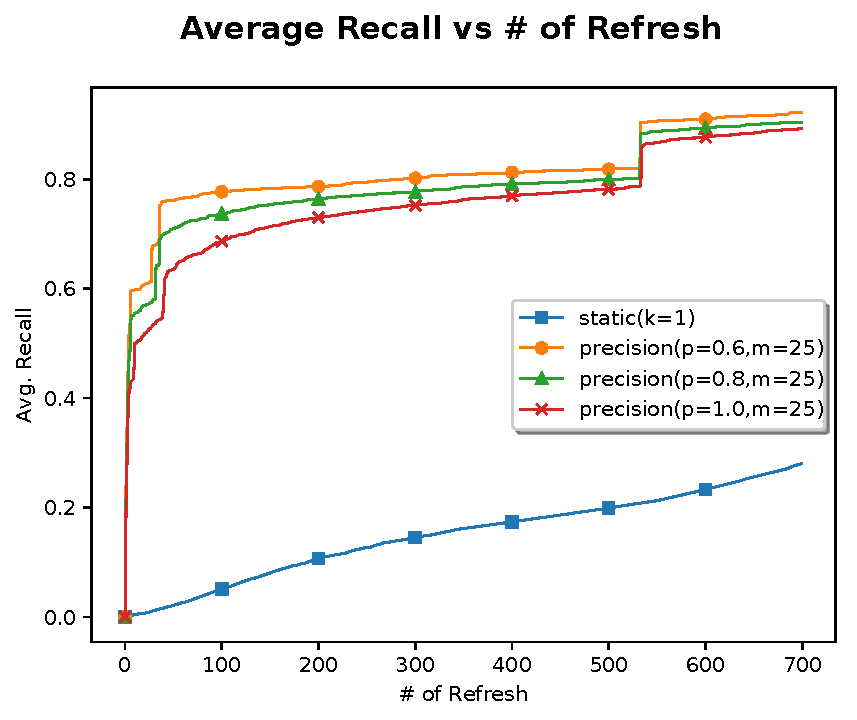
\includegraphics[width=1.0\linewidth]{prec2.pdf}
%  \caption{Precision Based Refresh}
%  \label{fig.prec2}
% \end{figure}

% \begin{figure}
%  \centering 
%  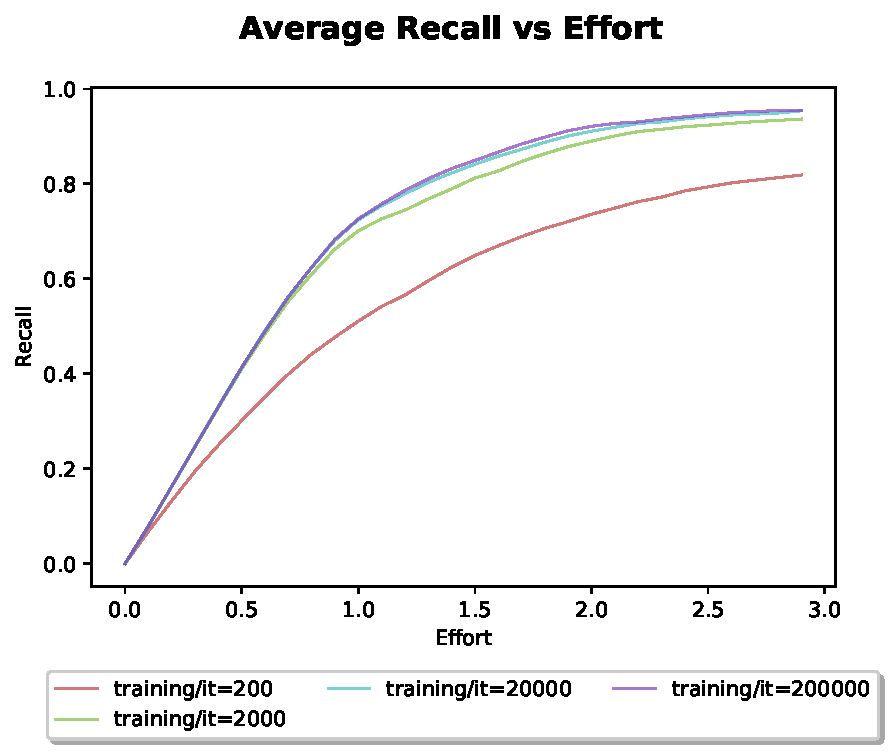
\includegraphics[width=1.0\linewidth]{train1.pdf}
%  \caption{Effect of number of training iterations}
%  \label{fig.train1}
% \end{figure}

% \begin{figure}
%  \centering 
%  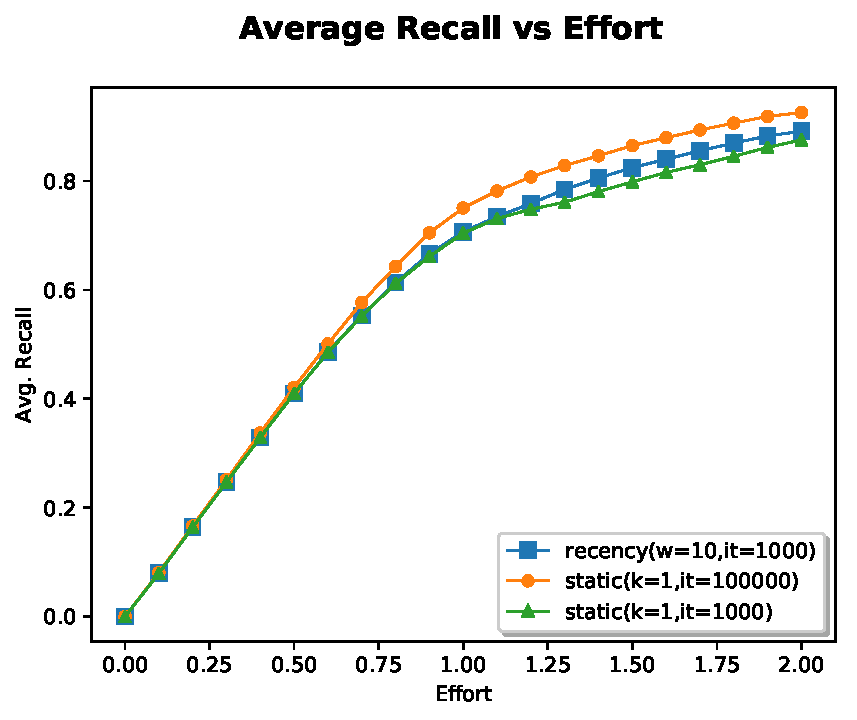
\includegraphics[width=1.0\linewidth]{rec1.pdf}
%  \caption{Recency Weighting}
%  \label{fig.recency1}
% \end{figure}
